\chapter{Introduction}
\label{chapter:introduction}
%\addcontentsline{toc}{chapter}{Introduction}
%\chaptermark{Introduction}

Dans ce premier chapitre, nous introduisons d'abord le contexte scientifique dans lequel s'inscrit cette thèse, puis le cadre de réalisation des travaux. Nous présentons ensuite les problématiques de recherche soulevées tout au long de la thèse, en donnant une vue à haut niveau de l'architecture considérée, et mettons en lien les contributions qui en ont émergé. Enfin, nous concluons par un résumé de l'organisation générale de ce document.

\section{Contexte scientifique}
%\addcontentsline{toc}{section}{Motivation}

En 1961, John McCarthy donne un discours pour célébrer les cent ans du MIT~\cite{greenberger1962management}. Il imagine alors que le partage du temps de calcul des ordinateurs pourrait permettre de vendre leur puissance d'exécution comme un service, à l'image de l'eau ou de l'électricité. Le matériel serait organisé de manière à rendre possible sa location à des clients qui paieraient ce service en fonction du volume, ou du temps d'utilisation.

Grâce à la démocratisation de l'accès à Internet à haut débit, au milieu des années 2000, l'idée de McCarthy se trouve mise en œuvre dans ce que l'on appelle \textit{cloud computing} (ou \textit{cloud}). Le cloud est un ensemble de services qui permettent d'utiliser des serveurs hébergés dans des centres de données, accessibles à distance, pour y déporter l'exécution de tout ou partie de diverses applications et y stocker des données~\cite{hayesCloudComputing2008}. Entreprises et particuliers peuvent dorénavant réduire drastiquement les coûts associés à l'achat et à l'entretien du matériel nécessaire au fonctionnement de leurs applications, en déléguant la responsabilité de l'infrastructure à des fournisseurs de services, qui bénéficient d'effets d'économie d'échelle en concentrant ces ressources dans d'immenses centres de données. Le cloud est parfois représenté dans un \textit{continuum} appelé \textit{cloud-edge}~\cite{jansenSPECRGReferenceArchitecture2023} : l'edge correspond à la périphérie du réseau, où les ressources de calcul et de stockage, limitées, sont déployées au plus proche des utilisateurs. Le cloud est un environnement distant au sein duquel les ressources sont disponibles dans de très grands volumes. Ces deux environnements peuvent être exploités de manière complémentaire.

Le premier modèle de service pour le cloud, encore aujourd'hui le plus répandu, est appelé \textit{Infrastructure as a Service} (IaaS) : les clients louent et réservent une sous-partie des ressources du fournisseur (processeurs, mémoire, stockage, réseau) dont ils deviennent responsables du fonctionnement~\cite{mellNISTDefinitionCloud}. Dans ce modèle, le client est intégralement en charge du dimensionnement des ressources dédiées à son application ; il pourra avoir tendance à surestimer ses besoins en ressources, de manière à s'assurer que l'application déployée soit capable d'absorber la montée en charge lors de pics d'activité~\cite{takMoveNotMove}. De nouvelles évolutions sont apparues au fil des années avec pour objectif de diminuer la surface des responsabilités du client. Par exemple, dans le modèle \textit{Platform as a Service} (PaaS), les clients n'ont pas directement accès aux ressources matérielles qui supportent leurs applications, et effectuent la plupart des tâches de gestion via des interfaces spécialisées. Ici, lorsque l'application n'est pas utilisée, elle reste toutefois déployée et occupe donc des ressources matérielles. Enfin, dans une offre \textit{Software as a Service} (SaaS), le fournisseur de services héberge et administre des applications, pour lesquelles il facture au client le droit d'en être utilisateur. Cette facturation est souvent forfaitaire, quelle que soit l'utilisation faite de l'application par le client.

Dans ces trois modèles traditionnels (IaaS, PaaS, SaaS), le client paie pour des ressources qui sont parfois dormantes. En effet, la mesure de l'usage du service s'effectue dans chacun des cas sur la quantité de ressources engagées pour sa mise en œuvre par le fournisseur. C'est un problème largement documenté dans la littérature, qui considère que le taux d'usage des ressources de calcul dans un centre de données cloud peut être inférieur à 15\% en moyenne~\cite{vasanWorthTheirWatts2010, vermaLargescaleClusterManagement2015a}.

Cette valeur faible est expliquée par un ensemble de facteurs. D'abord, une part du matériel disponible dans un centre de données est déployée pour palier les éventuelles pannes -- celles-ci peuvent affecter 3\% des machines chaque semaine~\cite{BareMetal70B}. Ensuite, un centre de données est toujours dimensionné par rapport aux pics d'utilisation, qui peuvent être liés à des événements récurrents comme le Super Bowl aux États-Unis~\cite{wangTouchdownCloudImpact2019}, ou imprévisibles comme la crise sanitaire de 2020~\cite{alashhabImpactCoronavirusPandemic2021} : c'est une marge de sécurité, permettant d'assurer la continuité du service. Enfin, le cloud est un secteur économique qui connaît une croissance soutenue -- autour de 15 à 20\% par an d'ici à la fin de la décennie selon plusieurs analystes~\cite{CloudComputingMarket, WorldwideSpendingPublic} -- ce qui explique des investissements réguliers dans du nouveau matériel pour tenir compte d'une éventuelle future demande.

Malgré tout, lorsque l'on met ce faible usage des ressources en regard de la consommation d'énergie estimée pour ces même centres de données, soit environ 1,5\% de la consommation d'électricité mondiale en 2010~\cite{masanetRecalibratingGlobalData2020}, ou jusqu'à 4\% de la demande totale dans l'Union Européenne~\cite{Electricity2024Analysis2024} en 2022, il semble urgent de s'intéresser à l'optimisation des opérations cloud.

En effet, l'accroissement de l'efficacité des architectures matérielles et logicielles n'a pas permis de contrer un certain effet rebond : si le rapport, pour un serveur typique du cloud, entre énergie consommée et calculs effectués a été divisé par quatre entre 2010 et 2020~\cite{masanetRecalibratingGlobalData2020}, la demande en matériel ne cesse de croître, poussée notamment par les immenses besoins en apprentissage machine~\cite{commentMetaOperate6002024}. Les investissements cumulés des leaders du secteur en serveurs dédiés à l'intelligence artificielle (IA) pourraient quintupler entre 2022 et 2025~\cite{DerriereIADeferlante2024, elderNextWaveAI2024}. L'Agence Internationale de l'Énergie (AIE) estime que la consommation des centres de données pourrait doubler d'ici à 2026~\cite{Electricity2024Analysis2024}, pour atteindre 6\% de la demande globale en électricité.

Une métrique couramment utilisée pour mesurer l'efficacité énergétique d'un centre de données est le PUE (\textit{Power Usage Effectiveness}). Cet indicateur mesure le rapport entre l'énergie totale engagée par le centre de données et l'énergie engagée pour le calcul (processeurs, mémoire, stockage, réseau), et devrait donc tendre vers $1$ dans l'idéal. En 2022, le PUE moyen se situe autour de 1,55~\cite{davisUptimeInstituteGlobal2022}, principalement gonflé par les besoins en refroidissement des machines. Cet écart pèse sur les coûts d'exploitation et représente un manque à gagner pour les fournisseurs de services.
% Pourtant, un serveur éteint n'a pas besoin d'être refroidi. Comment expliquer alors que les ressources matérielles restent dans un état de stase, augmentant la consommation des centres de données sans générer de revenus ? Serait-il possible d'envisager un modèle dans lequel les ressources sont allouées au plus proche des besoins, laissant la possibilité aux fournisseurs de services de mettre en œuvre des politiques d'extinction pour les serveurs inutilisés ?

Au cours des années 2010, des acteurs du cloud public ont proposé une nouvelle déclinaison de leur offre commerciale, le modèle \textit{Function as a Service} (FaaS). En particulier, Amazon a lancé Lambda~\footnote{\href{https://aws.amazon.com/fr/lambda/}{https://aws.amazon.com/fr/lambda/}} en 2014. Avec Lambda, Amazon propose à ses clients de décomposer leurs applications en un ensemble de fonctions les plus simples possibles. Cette décomposition permet de mettre à l'échelle les ressources allouées à l'application à la granularité la plus fine, ce qui permet de mesurer l'usage du service au plus près de l'usage réel des ressources et d'adapter la facturation en fonction du trafic reçu par l'application.

Le modèle FaaS est une mise en œuvre particulière d'un paradigme plus général pour le cloud que l'on nomme \textit{serverless computing}, ou \textit{serverless}~\cite{hellersteinServerlessComputingOne2019}. Dans ce paradigme, la granularité de réservation des ressources se déplace de la \textit{quantité} vers la \textit{durée} : les clients fournissent le code qu'ils souhaitent exécuter sur la plateforme cloud, et les ressources nécessaires à cette exécution sont allouées \textit{lorsque} nécessaire, et \textit{autant} que nécessaire, c'est-à-dire à la hauteur des requêtes utilisateur reçues par l'application. Tant que l'application est inutilisée, les ressources sont libérées. Dès que la charge augmente, les ressources allouées augmentent pour absorber le trafic.

Le cadre des travaux de cette thèse est celui de l'\textit{orchestration}. Dans le paradigme serverless, l'orchestration est le mécanisme de placement des tâches. Ce mécanisme est dual et dynamique : il recouvre l'\textit{allocation} des ressources et l'\textit{ordonnancement} des requêtes utilisateur~\cite{vaneykSPECRGReferenceArchitecture2019}, et se déroule \textit{en ligne}, c'est-à-dire lors du déploiement des applications. L'allocation consiste à dimensionner les ressources matérielles affectées à une application, et l'ordonnancement consiste à placer les requêtes utilisateur en file d'attente sur ces ressources préalablement allouées. L'enjeu pour le fournisseur de services est de réaliser cette orchestration en maintenant un niveau de performances acceptable pour les applications déployées. Car dans le cloud, fournisseurs de services et clients sont souvent liés par des accords de niveau de service (SLA, pour \textit{Service Level Agreement}) : ces contrats stipulent des objectifs de niveau de service (SLO, pour \textit{Service Level Objective}) au regard de métriques de performances (latence, débit, etc.) qui déterminent la qualité de service (QoS, pour \textit{Quality of Service}). Lorsque ces contrats ne sont pas respectés, le fournisseur est généralement tenu de verser des pénalités sous la forme de remises ou de remboursements à ses clients~\cite{buyyaSLAorientedResourceProvisioning2011}. C'est une des raisons pour lesquelles les centres de données sont dimensionnés en fonction des pics d'activité.

Le déplacement de la responsabilité du dimensionnement des ressources allouées aux applications du client vers le fournisseur de services ouvre de nouvelles possibilités d'optimisation pour ce dernier, en appliquant des stratégies intelligentes de gestion des ressources. D'une part, cela lui permet de garantir un niveau satisfaisant de qualité de service pour les clients, et donc d'éviter le paiement de pénalités lorsque les accords de niveau de service sont violés. D'autre part, alors que le coût de la consommation électrique d'un serveur pendant son cycle d'exploitation dépasse aujourd'hui son prix d'achat~\cite{orgerieSurveyTechniquesImproving2014}, il semble opportun de profiter de ce contrôle accru pour limiter cette consommation. % Par ailleurs, sur les aspects réglementaires, de nouvelles exigences émergent en matière de mesure de la consommation d'énergie et de l'empreinte carbone pour les opérateurs de centres de données~\cite{davisUptimeInstituteGlobal2022}. % La granularité offerte par le serverless devrait permettre aux fournisseurs de service une plus grande traçabilité sur les postes de consommation d'énergie au sein de leurs centres de données.

Il apparaît donc que le fournisseur de services a tout intérêt à optimiser l'orchestration des charges de travail dans ses centres de données. Si la granularité de l'allocation des ressources offerte par le paradigme serverless apparaît comme étant une solution toute trouvée aux problèmes d'usage des ressources dans le cloud, ce mécanisme induit un certain nombres de défis à relever~\cite{Lannurien2023}. Pour optimiser le processus d'orchestration, il faut prendre en compte la diversité des ressources à disposition : le cloud est un environnement hautement hétérogène, dans lequel cohabitent de nombreuses architectures matérielles qui présentent des niveaux de performances et de coût très divers~\cite{reissHeterogeneityDynamicityClouds}. Par ailleurs, il ne s'agit pas uniquement de proposer les performances les plus élevées de manière indiscriminée. Par exemple, de nombreux utilisateurs de services cloud n'ont pas besoin de garanties fortes en matière de latence~\cite{tirmaziBorgNextGeneration2020}. Ainsi, une connaissance fine des utilisateurs et des charges de travail est requise pour mettre en œuvre des politiques pertinentes de répartition de charge ou de consolidation des tâches, qui permettent une satisfaction \textit{au plus juste} des besoins des utilisateurs en matière de qualité de service.

\section{Cadre des travaux}

La thèse vise à concevoir un orchestrateur serverless, en prenant en compte l’hétérogénéité des ressources matérielles pour optimiser le placement des tâches dans le respect des accords de niveau de service, tout en minimisant la consommation d'énergie du système.

Cette thèse s'est conduite en partenariat entre le Lab-STICC et l'Institut de Recherche Technologique (IRT) b{\textless\textgreater}bcom~\footnote{\href{https://b-com.com/}{https://b-com.com/}}, créé en 2012. b{\textless\textgreater}bcom est l'un des huit IRT français. Son ambition est de fournir des solutions numériques au service des entreprises et de leur compétitivité. Il est particulièrement actif dans les domaines des télécommunications, de l'audiovisuel et de l'immersion.

Les travaux de cette thèse se sont inscrits dans deux projets au sein de l'IRT. Dans le cadre du projet SUPRA d'abord, qui entend livrer un système de cloud souverain pour les applications télécom, e-santé et intelligence artificielle sur des infrastructures en propre. Les travaux de thèse se sont poursuivis tout au long du projet RPC ensuite, un axe transversal à b{\textless\textgreater}com qui mobilise une grande partie des équipes, dans le but de concevoir un système souverain de radio logicielle (RAN, pour \textit{Radio Access Network}), déployé dans un environnement virtualisé et distribué entre cloud et edge.

\section{Problématiques de recherche}
%\addcontentsline{toc}{section}{Problématiques de recherche}

Cette section présente l'architecture générale du système considéré au cours de cette thèse ainsi que les hypothèses que nous avons formulées. Elle résume les problèmes que nous avons identifiés, et pose les questions de recherche que nous avons adressées dans le but de lever ces verrous.

\begin{figure}[h!]
    \centering
	%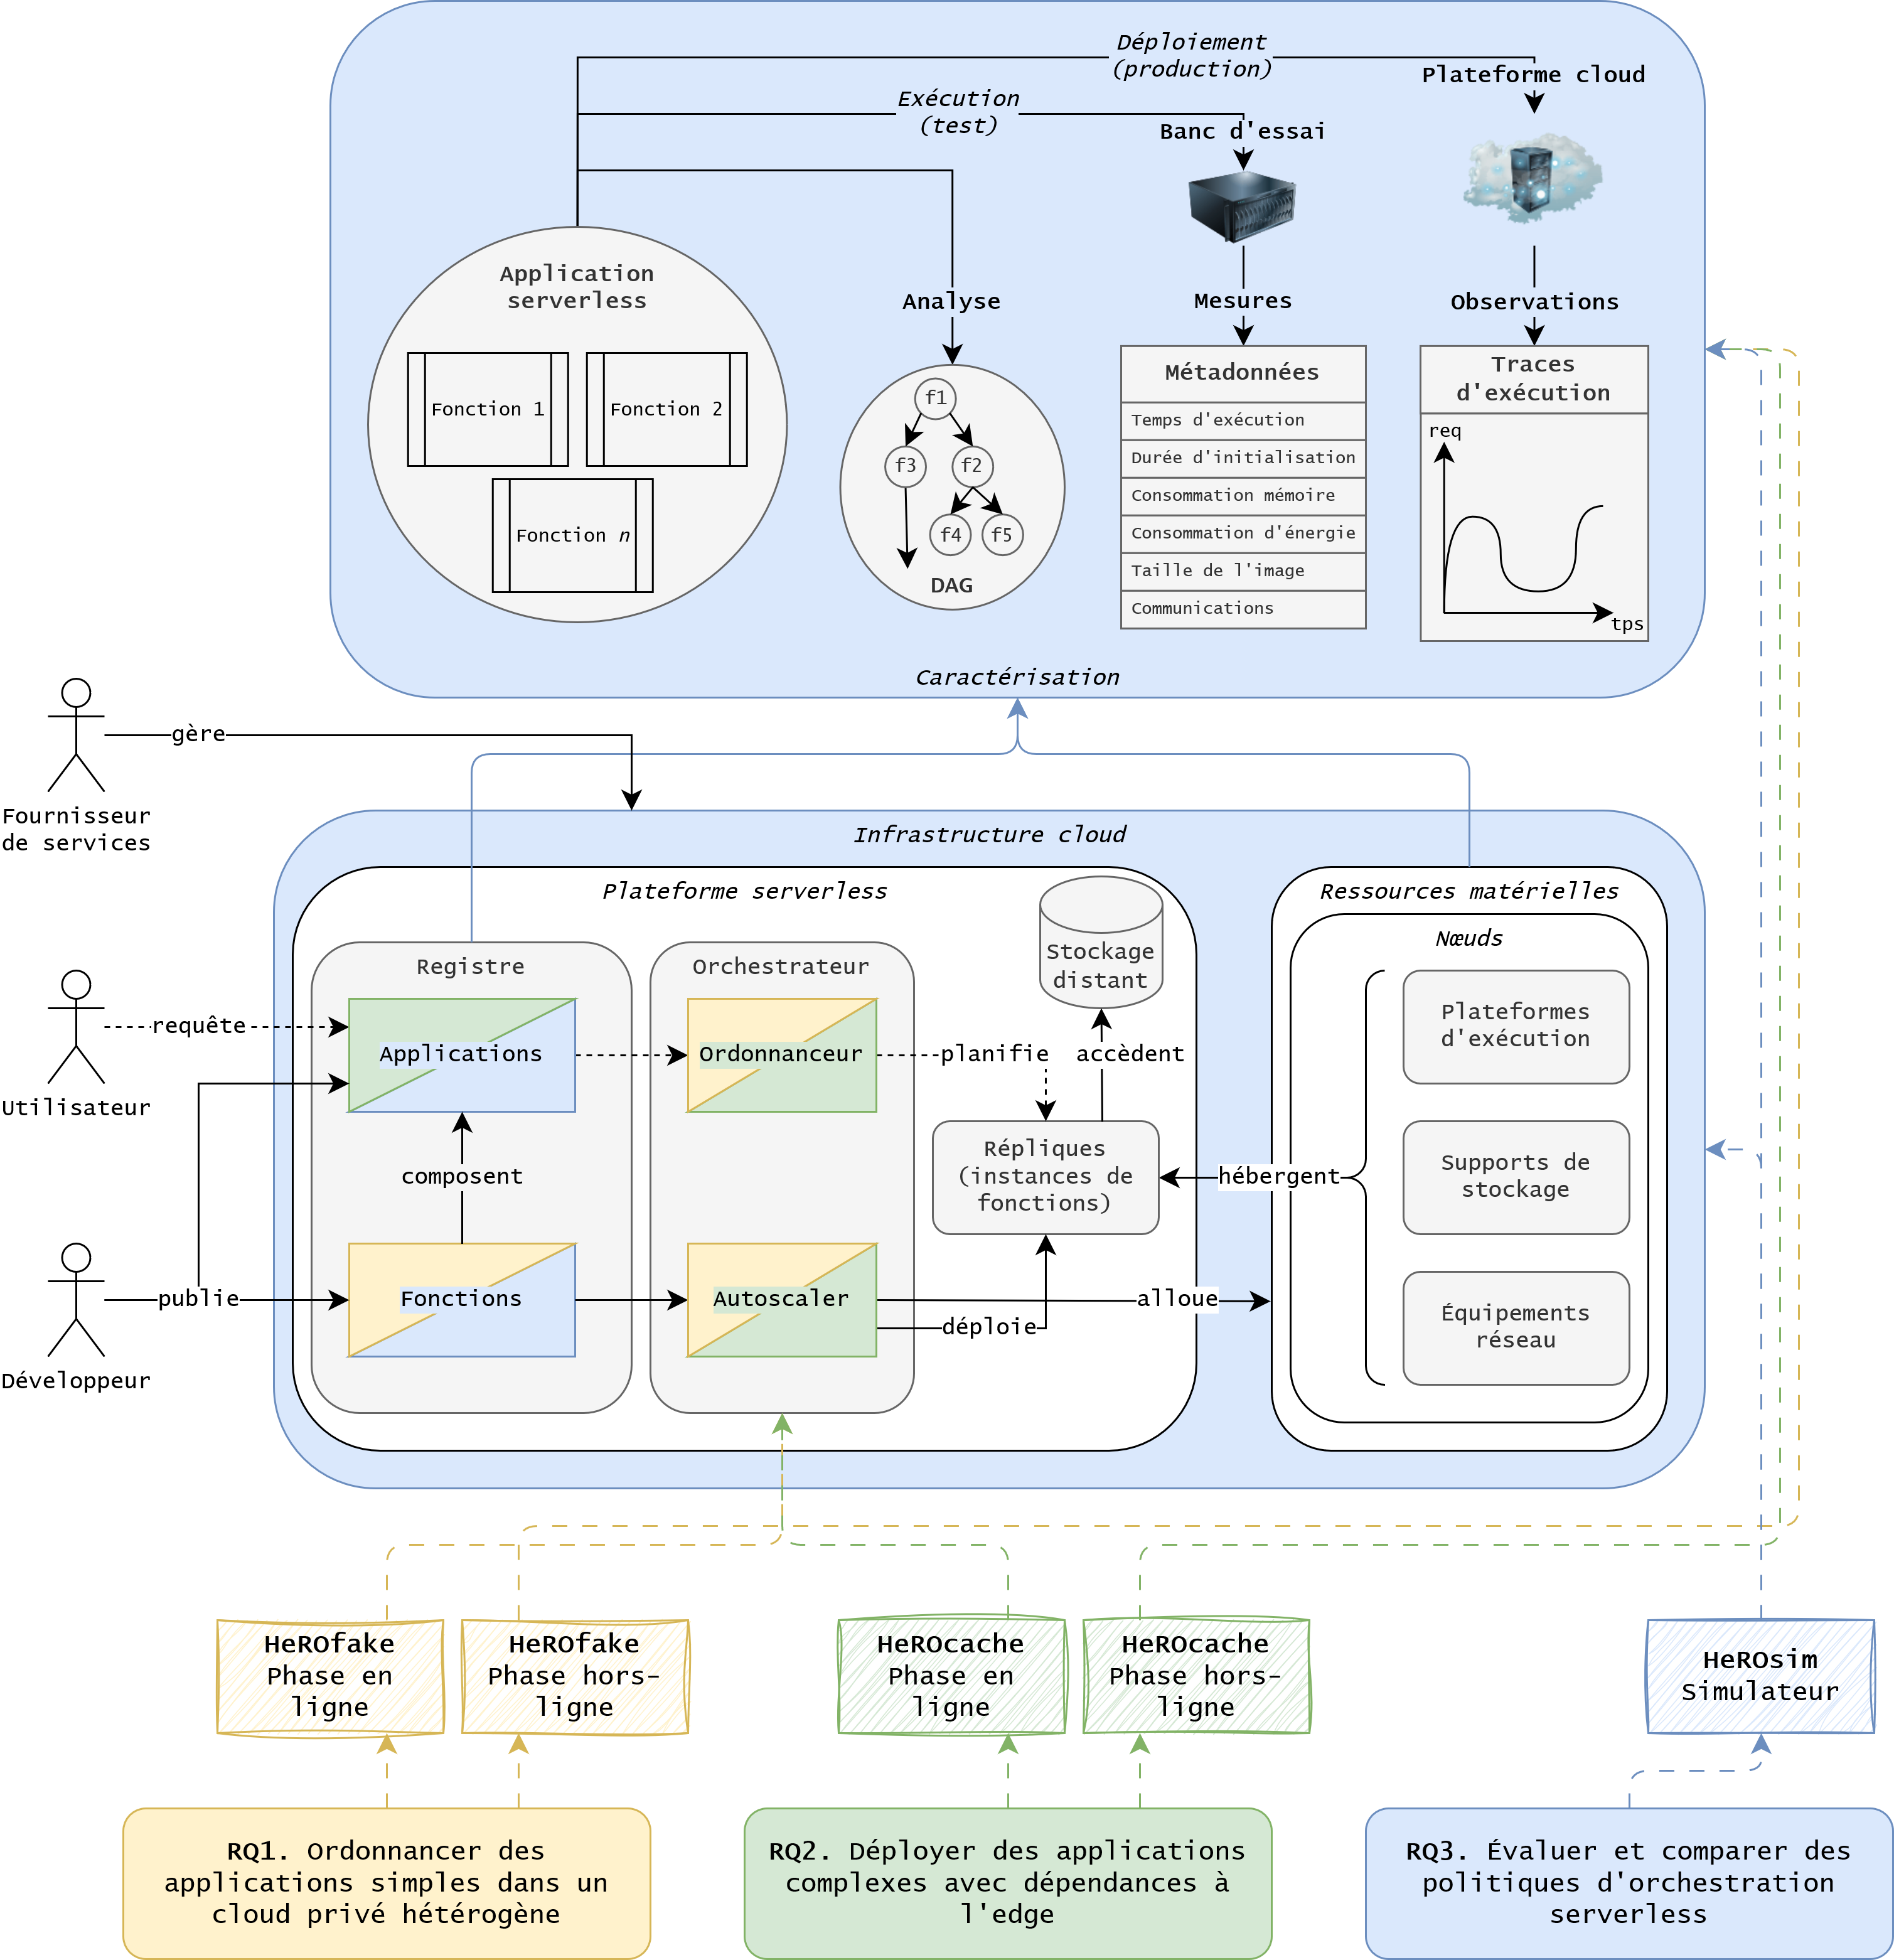
\includegraphics[width=\textwidth]{1_Introduction/figures/architecture.pdf}
    \includesvg[width=\textwidth]{1_Introduction/figures/architecture.svg}
	\caption{Vue à haut niveau de l'architecture considérée, en lien avec nos questions de recherche et nos contributions.}
	\label{fig:intro-architecture}
\end{figure}

Les travaux menés au cours de cette thèse s'inscrivent dans le cadre du modèle de service serverless pour le cloud. Nous avons considéré un environnement dans lequel un fournisseur de services dispose de ressources matérielles que des développeurs peuvent exploiter pour déployer leurs applications à destination d'une variété d'utilisateurs. % Nous avons cherché à concevoir une plateforme d'orchestration qui soit en mesure de garantir la qualité de service pour les utilisateurs tout en minimisant les coûts pour le fournisseur de services.
La figure~\ref{fig:intro-architecture} montre une vue générale de l'architecture du système considéré dans les travaux de cette thèse, ses liens avec nos questions de recherche, ainsi qu'un aperçu du positionnement des contributions au sein de cette architecture.

Les applications, les fonctions et les ressources matérielles sont considérées comme des données d'entrée dans nos contributions. Les applications sont définies par les développeurs ; elles comportent une à plusieurs fonctions, qui peuvent présenter des relations de dépendances (temporelles ou de données) que l'on exprime comme un graphe acyclique (DAG, pour \textit{Directed Acyclic Graph}). Les fonctions sont publiées par les développeurs, en vue d'être déployées par la plateforme serverless lors d'une requête utilisateur. Les ressources matérielles constituent l'ensemble des ressources de calcul (processeurs, mémoire, stockage, réseau) disponibles dans l'infrastructure fournisseur de services. Elles sont réparties au sein de plusieurs nœuds (des serveurs physiques dans le centre de données du fournisseur).

La plateforme serverless comporte une brique logicielle centrale appelée orchestrateur. L'orchestrateur est composé de deux éléments principaux : un \textit{autoscaler}, chargé de l'allocation des ressources matérielles nécessaires au déploiement des fonctions ; ainsi qu'un \textit{ordonnanceur}, responsable de la planification des requêtes utilisateur dans les files d'attente des répliques de fonctions. Les répliques sont des environnements d'exécution pour les instances des fonctions déployées par la plateforme serverless. Les requêtes utilisateur y sont placées en file d'attente avant traitement.

% Une progression s'est opérée, en partant de l'ordonnancement de fonctions simples (sans dépendances et sans état), pour arriver au déploiement d'applications complexes (dépendances temporelles et de données entre les fonctions des applications). Il nous a également fallu développer un environnement d'évaluation des différentes politiques que nous avons proposées.

\begin{center}
    \rule{4cm}{0.4pt}
\end{center}

\textbf{Problème 1} -- L'allocation de ressources au sein d'une plateforme serverless se fait sur un mode réactif, c'est-à-dire en réponse à une variation du trafic. Lorsque de nouvelles instances des fonctions doivent être déployées, cela provoque une latence additionnelle qui peut dégrader la qualité de service pour les utilisateurs. Le problème est particulièrement saillant dans l'environnement hautement hétérogène qu'est celui du cloud : les ressources matérielles ont différents niveaux de performances et de coût ; les applications interactives (c'est-à-dire dirigée par les évènements, par opposition à une application par lots) présentent des motifs d'usage difficilement prédictibles ; et les utilisateurs ont des besoins irréguliers et variés en qualité de service.

\boitemagique{Question 1 (\textbf{QR1})}{
    Comment dimensionner les allocations dynamiques de ressources hétérogènes pour une application simple, constituée de fonctions sans dépendances, et comment ordonnancer efficacement les requêtes utilisateur, lorsque ces derniers ont des besoins variés en matière de qualité de service ?
}

\begin{center}
    \rule{4cm}{0.4pt}
\end{center}

\textbf{Problème 2} -- Ordonnancer des applications complexes, constituées d'un ensemble de fonctions qui présentent des relations de dépendances et communiquent entre elles des résultats intermédiaires, soulève un problème lié au stockage dans le modèle serverless. En effet, les solutions commerciales s'appuient sur un \textit{stockage distant}, partagé entre les utilisateurs et accédé par le réseau. Ce stockage présente des performances limitées et parfois imprévisibles, notamment du point de vue de la latence, ce qui peut provoquer des délais à chaque étage de l'application. Ces délais s'accumulent alors et provoquent un effet boule de neige, dégradant drastiquement la qualité de service. Par opposition, une possibilité existe d'exploiter le \textit{stockage local} aux nœuds de calcul, c'est-à-dire les supports de stockage physiquement installés sur les serveurs. Mais cela induit un risque de contention sur les ressources, qui peuvent être limitées en capacité et en performances dans le cadre de l'informatique en périphérie (ou \textit{edge}).

\boitemagique{Question 2 (\textbf{QR2})}{
    Comment déployer des applications complexes, composées de chaînes de fonctions de courte durée, et comment tirer parti de l'hétérogénéité des nœuds disponibles à l'edge, pour respecter la qualité de service requise par les utilisateurs tout en contenant la consommation d'énergie de l'infrastructure ?
    % Comment prendre en compte les délais d'initialisation et de communications lorsque l'on déploie des chaînes de fonctions de courte durée, et comment tirer parti de l'hétérogénéité des nœuds à disposition, pour respecter la qualité de service requise par les utilisateurs et contenir la consommation d'énergie de l'infrastructure ?
}

\begin{center}
    \rule{4cm}{0.4pt}
\end{center}

\textbf{Problème 3} -- Évaluer des politiques d'orchestration pour un environnement cloud peut se faire de deux manières différentes : par expérimentation, c'est-à-dire avec du matériel et des utilisateurs réels, ou en simulation. La méthode empirique se heurte à des contraintes de coût d'une part, car il faut réserver une partie de l'infrastructure pour mener les campagnes de mesure. D'autre part, il est complexe d'explorer des scénarios hypothétiques en production, c'est-à-dire de se laisser la liberté de changer un certain nombre de paramètres en entrée pour évaluer leur impact (fréquence des requêtes, caractéristiques du matériel, etc.). Une seconde méthode consiste à modéliser l'environnement cible en s'appuyant sur des simulateurs à l'état de l'art pour le cloud qui, quant à eux, présentent des limites qui rendent délicate la représentation fidèle d'un environnement serverless permettant de comparer les performances de différentes stratégies de gestion des ressources.

\boitemagique{Question 3 (\textbf{QR3})}{
    Du point de vue d'un fournisseur de services pour le cloud, comment évaluer et comparer l'impact sur la qualité de service de différentes politiques d'allocation de ressources et d'ordonnancement de tâches dans le modèle serverless ?
}

\section{Contributions}
%\addcontentsline{toc}{section}{Contributions}

Cette section présente les trois contributions principales de la thèse, en indiquant comment elles s'articulent autour des trois questions de recherche précédemment énoncées.

\subsection{Caractérisation et orchestration d'applications simples pour la détection de deepfake}

La \textbf{QR1} (\textit{dimensionnement et ordonnancement sur ressources hétérogènes}) a émergé d'une réflexion autour du déploiement d'une application sensible à la latence sur des ressources non-réservées au sein de l'IRT b{\textless\textgreater}com. Notre cas d'étude concerne une application de détection de deepfake -- des images ou des vidéos générées numériquement dans un but malicieux, avec l'objectif de tromper leur destinataire en représentant des situations ou des discours qui n'ont pas existé dans la réalité~\cite{westerlundEmergenceDeepfakeTechnology2019}. Cette application est réveillée par l'envoi, par un utilisateur, d'une image à classifier. Elle s'appuie sur des algorithmes d'apprentissage machine pour déterminer si l'image est en effet synthétique ou bien réelle.

\sloppy Pour répondre à la \textbf{QR1}, nous avons proposé HeROfake (pour \textit{\textbf{He}terogeneous \textbf{R}esources \textbf{O}rchestration for deep\textbf{fake} detection}, voir chapitre~\ref{chapter:herofake}), une plateforme d'orchestration serverless qui vise à réaliser de manière intelligente l'allocation des ressources et l'ordonnancement des requêtes, dans le but d'optimiser l'orchestration pour la qualité de service tout en minimisant la consommation d'énergie du système. Nous avons mené une campagne de mesures afin de caractériser l'exécution d'un ensemble de fonctions d'inférence, utilisées par l'application et basées sur des réseaux de neurones, sur un ensemble de ressources matérielles hétérogènes (CPU, GPU, FPGA). Cette phase de caractérisation permet d'obtenir des métadonnées sur le niveau de performances et de consommation de ressources pour l'application.

Ces métadonnées sont ensuite utilisées par l'orchestrateur lors d'une phase en ligne, afin d'ajuster ses décisions d'allocation et d'ordonnancement tout au long d'un scénario, rejoué en simulation dans un environnement ad-hoc. Nous avons établi un modèle de coût pour cet orchestrateur, puis conçu une politique d'optimisation multiobjectif visant à minimiser ces fonctions de coût, nourries par les métadonnées issues de la phase de mesures.

Cette contribution a fait l'objet d'une publication dans la conférence \textbf{IEEE/ACM 23rd International Symposium on Cluster, Cloud and Internet Computing} (CCGrid, 2023)~\cite{herofake}.

\subsection{Modèle de coût pour l'orchestration serverless d'applications complexes à l'\textit{edge}}

La \textbf{QR2} (\textit{prise en compte des coûts associés au stockage dans le serverless}) a émergé pour deux raisons principales. D'une part, comme la suite logique des travaux menés sur la première contribution : si notre précédente contribution permet d'orchestrer des fonctions sans état, nous savons que la plupart des applications ont besoin de stocker des données intermédiaires pendant leur exécution. D'autre part, une étude de la littérature en matière d'orchestration serverless nous a permis de constater que de nombreuses contributions prenaient souvent comme point de départ une situation très favorable, considérant que les images servant à déployer les fonctions sont toujours disponibles sur les nœuds de calcul, et que les communications entre les fonctions sont transparentes du point de vue des performances.

Pour répondre à la \textbf{QR2}, nous avons cherché à établir un modèle de coût pour l'allocation de ressources et l'ordonnancement des tâches qui prenne en compte ces deux mécanismes liés au stockage. Notre cas d'étude pour cette contribution est une application de détection d'instrusions, déployée à l'edge, sur des nœuds hétérogènes aux ressources contraintes et limités en nombre par l'énergie disponible. Nous avons proposé HeROcache (pour \textit{\textbf{He}terogeneous \textbf{R}esources \textbf{O}rchestration with a \textbf{cache} strategy}), voir chapitre~\ref{chapter:herocache}), une stratégie d'orchestration qui cherche à maximiser la consolidation des fonctions d'une même application sur les mêmes nœuds, afin de minimiser la consommation d'énergie de l'infrastructure. Grâce à un mécanisme de mise en cache des données sur le stockage local, cette stratégie permet de réduire les délais de communication des applications et limite les violations de qualité de service.

Cette contribution a fait l'objet d'une publication dans la conférence \textbf{IEEE/ACM 24rd International Symposium on Cluster, Cloud and Internet Computing} (CCGrid, 2024)~\cite{herocache}.

\subsection{Simulation à événements discrets pour l'évaluation de politiques d'orchestration}

% données de production (traces d'exécution), analyse (graphe des appels, données intermédiaires), caractérisation (métriques de performances)

La \textbf{QR3} (\textit{évaluer et comparer différentes politiques d'orchestration serverless}) a été transversale tout au long des travaux de thèse. Concevoir des stratégies d'allocation et d'ordonnancement pour le cloud demande d'avoir à notre disposition un environnement dans lequel les évaluer.

Pour répondre à la \textbf{QR3}, nous avons développé et proposé HeROsim (pour \textit{\textbf{He}terogeneous \textbf{R}esources \textbf{O}rchestration \textbf{sim}ulator}, voir chapitre~\ref{chapter:herosim}), un simulateur \textit{open source} à événements discrets pour le cloud serverless, qui présente les caractéristiques nécessaires à la modélisation fine d'un environnement serverless et l'évaluation de politiques d'orchestration. La simulation progresse à une granularité au niveau d'une requête utilisateur, et permet de modéliser des applications complexes (dépendances entre les fonctions) et des environnements hétérogènes (nœuds à différents niveaux de performances, requêtes à différents niveaux de qualité de service). HeROsim permet de rejouer des scénarios (sur la base de traces d'exécution) et de comparer les résultats de différentes politiques au regard de métriques de qualité de service et de consommation d'énergie.

Cette contribution a fait l'objet d'une soumission au journal \textbf{IEEE Internet Computing}~\cite{herosim} en mai 2024.

\clearpage

\section{Organisation de la thèse}
%\addcontentsline{toc}{section}{Organisation du mémoire}

Ce manuscrit est composé de sept chapitres (dont cette introduction), organisés comme suit :

\begin{center}
    \rule{4cm}{0.4pt}
\end{center}

\textbf{Partie~\ref{part:one} : Contexte et état de l'art}

Le chapitre~\ref{chapter:context} décrit l'environnement général des travaux de la thèse, et donne en particulier les caractéristiques du cloud et du modèle serverless. Le chapitre~\ref{chapter:sota} présente des contributions de l'état de l'art dans le domaine de l'orchestration dynamique pour le cloud.

\begin{center}
    \rule{4cm}{0.4pt}
\end{center}

\textbf{Partie~\ref{part:two} : Contributions}

Cette partie présente les trois contributions de la thèse. Le chapitre~\ref{chapter:herofake} décrit notre solution d'allocation et d'ordonnancement dynamiques sous contrainte de qualité de service pour des fonctions simples, ainsi que notre méthodologie de caractérisation des plateformes et des tâches. Le chapitre~\ref{chapter:herocache} présente notre orchestrateur s'appuyant sur un modèle de coût intégrant les problématiques de stockage pour le serverless. Le chapitre~\ref{chapter:herosim} détaille l'environnement de simulation développé dans le cadre de la thèse pour évaluer des politiques d'orchestration serverless pour le cloud.

\begin{center}
    \rule{4cm}{0.4pt}
\end{center}

\textbf{Partie~\ref{part:three} : Conclusion et perspectives}

Enfin, le chapitre~\ref{chapter:conclusion} résume les contributions de la thèse et présente les limites identifiées dans les solutions proposées, pour ouvrir la discussion sur des perspectives de futurs travaux.
